%%%%%%%%%%%%%%%%%%%%%%%%%%%%%%%%%%%%%%%%%
% Journal Article
% LaTeX Template
% Version 1.4 (15/5/16)
%
% This template has been downloaded from:
% http://www.LaTeXTemplates.com
%
% Original author:
% Frits Wenneker (http://www.howtotex.com) with extensive modifications by
% Vel (vel@LaTeXTemplates.com)
%
% License:
% CC BY-NC-SA 3.0 (http://creativecommons.org/licenses/by-nc-sa/3.0/)
%
%%%%%%%%%%%%%%%%%%%%%%%%%%%%%%%%%%%%%%%%%

%----------------------------------------------------------------------------------------

%	PACKAGES AND OTHER DOCUMENT CONFIGURATIONS
%----------------------------------------------------------------------------------------
\documentclass[twoside,twocolumn]{article}

\usepackage[sc]{mathpazo} % Use the Palatino font
\usepackage[T1]{fontenc} % Use 8-bit encoding that has 256 glyphs
%\linespread{1.05} % Line spacing - Palatino needs more space between lines
\usepackage{microtype} % Slightly tweak font spacing for aesthetics

\usepackage[english]{babel} % Language hyphenation and typographical rules

\usepackage[hmarginratio=1:1,top=32mm,columnsep=20pt]{geometry} % Document margins
\usepackage[hang, small,labelfont=bf,up]{caption} % Custom captions under/above floats in tables or figures
\usepackage{booktabs} % Horizontal rules in tables

\usepackage{lettrine} % The lettrine is the first enlarged letter at the beginning of the text

\usepackage{enumitem} % Customized lists
\setlist[itemize]{noitemsep} % Make itemize lists more compact

\usepackage{abstract} % Allows abstract customization
\renewcommand{\abstractnamefont}{\normalfont\bfseries} % Set the "Abstract" text to bold
\renewcommand{\abstracttextfont}{\normalfont\small\itshape} % Set the abstract itself to small italic text

\usepackage{titlesec} % Allows customization of titles
\renewcommand\thesection{\Roman{section}} % Roman numerals for the sections
\renewcommand\thesubsection{\roman{subsection}} % roman numerals for subsections
\titleformat{\section}[block]{\large\scshape\centering}{\thesection.}{1em}{} % Change the look of the section titles
\titleformat{\subsection}[block]{\large}{\thesubsection.}{1em}{} % Change the look of the section titles

\usepackage{fancyhdr} % Headers and footers
%\pagestyle{fancy} % All pages have headers and footers
%\fancyhead{} % Blank out the default header
%\fancyfoot{} % Blank out the default footer
%\fancyhead[C]{Running title $\bullet$ May 2016 $\bullet$ Vol. XXI, No. 1} % Custom header text
%\fancyfoot[RO,LE]{\thepage} % Custom footer text

\usepackage{titling} % Customizing the title section

\usepackage{hyperref} % For hyperlinks in the PDF

\usepackage{graphicx}
\usepackage[tbtags]{amsmath}

%----------------------------------------------------------------------------------------
%	TITLE SECTION
%----------------------------------------------------------------------------------------

\setlength{\droptitle}{-4\baselineskip} % Move the title up

\pretitle{\begin{center}\Huge\bfseries} % Article title formatting
\posttitle{\end{center}} % Article title closing formatting
\title{Modeling Damped Oscillations} % Article title
\author{%
\textsc{Tian Ye} \\%\thanks{A thank you or further information} \\[1ex] % Your name
\normalsize Henry Samueli School of Engineering and Applied Science, Univ. California Los Angeles \\ % Your institution
\and % Uncomment if 2 authors are required, duplicate these 4 lines if more
\textsc{Chris Ong} \\%\thanks{Corresponding author} \\[1ex] % Second author's name
\normalsize College of Letters and Science, Univ. California Los Angeles \\ % Second author's institution
%\normalsize \href{mailto:jane@smith.com}{jane@smith.com} % Second author's email address
}
\date{November 7, 2017} % Leave empty to omit a date
\renewcommand{\maketitlehookd}{%
\begin{abstract}
\noindent In Classical Physics, an oscillation is described as the periodic motion of a body about an equilibrium position. A simple harmonic oscillation is defined as when the only force acting on the oscillator is the restoring force that is directly proportional to displacement of the oscillator from equilibrium. Both amplitude and frequency of oscillation remain constant in an ideal simple harmonic oscillator. When a second force that is proportional to the velocity is acting on the body, it is known as a damped oscillation. This lab aims to analyze the frequencies of an undamped and damped oscillation. The damping of the oscillation  is accomplished via dropping a magnetized weight into an aluminum tube. The subsequent eddy currents produced by the change of magnetic flux within the pipe and the subsequent dissipation of heat due to the resistivity of the aluminum within the pipe serve as the source of the damping force. The predicted frequency of oscillation is $(0.693 \pm 0.006)$ Hz and the calculated frequencies of oscillation for the undamped and damped oscillations are $(0.6936 \pm 0.0002)$ Hz and $(0.6926 \pm 0.0018)$Hz, respectively. All values fall within their uncertainties of each other.
\end{abstract}
}

%----------------------------------------------------------------------------------------

\begin{document}

% Print the title
\maketitle

%----------------------------------------------------------------------------------------
%	ARTICLE CONTENTS
%----------------------------------------------------------------------------------------

\section{Introduction}

This report discusses the resonance frequencies of a damped and undamped harmonic oscillator. The objective is to model the damping of the oscillation using Equation 5.2 and to solve for the damping time using Equation 5.7 from the Lab Manual, listed as Equation 1 and Equation 2 below, respectively.

\footnotesize
\begin{align}
m\ddot{x}&= -kx - b\dot{x} \\
\tau &\equiv \frac{2m}{b}
\end{align}
\normalsize

Where $k$ is the spring constant, $x$ is the position of the hanging weight in the vertical direction, $m$ is the mass of the weight, and $b$ is the damping term.$\textsuperscript{[1]}$  It is interesting to note that while harmonic oscillators are nearly as ubiquitous as the force of friction, there nonetheless still has yet to exist a simple solution to the modeling of the force of friction in a damped harmonic system.$\textsuperscript{[2]}$

%------------------------------------------------

\section{Methods}

The first portion of the experiment involves solving for the spring constant $k$ by massing 5 different weights before attaching them to the bottom of the spring and measuring the distance of the stretched spring from the ground. $k$ is then solved by plotting force (obtained by multiplying the masses by the gravitational constant) against displacement and fitting a line to the slope.

\hfill

\noindent A force sensor is then set up on a stand in a vertical orientation so that the hook is on the bottom end of the sensor. Strings are tied to both ends of the spring, which then connect the spring to the force sensor on one end and a mass with magnets within it on the other end. The strings are used to eliminate systematic uncertainty due to the potential rotation of the spring as it stretches and compresses. The force sensor is then connected to PASCO and set up to display voltage, with a sample rate of 40 Hz. 

\hfill

\noindent For the undamped oscillation, the spring is set into a small amplitude oscillation to minimize noise; Capstone then records the voltage vs time data for 20 seconds. For the damped oscillation, the same procedure is repeated with exception that the mass is placed inside an aluminum tube so that the oscillation is contained entirely within it without touching the tube itself.

%------------------------------------------------

\section{Analysis}

To solve for $k$, we hang several masses from the spring and record the distance from the floor the spring stretches to. We then convert the mass to force by multiplying the mass by the gravitational constant, 9.8 m/s$^2$, and plot the data.

\begin{figure}[!htbp]
    \centering
    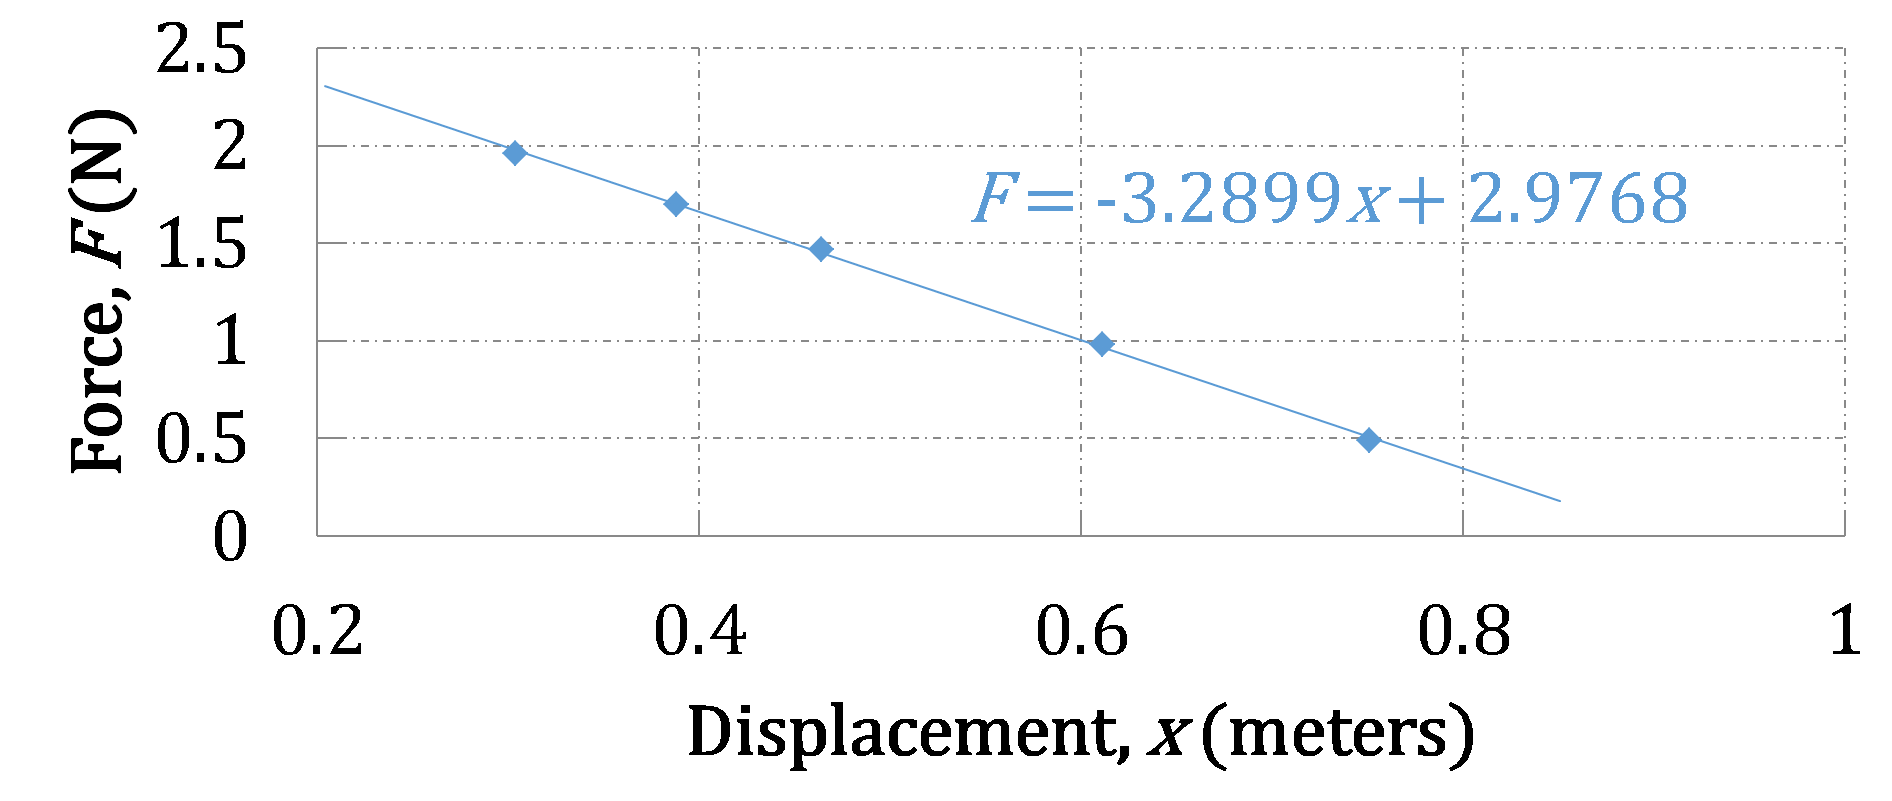
\includegraphics[width=2.9in]{SpringConst.png}
    \caption{\textit{Solving for spring constant.} The blue line is a linear fit to the data, $F = kx + N$, with fit parameters of $k$ = (-3.2899 $\pm$ 0.0537) N/m and $N$ = (2.9768 $\pm$ 0.0283) N.}
\end{figure}

\noindent Since the spring constant $k$ is a relationship between force and displacement, we can determine $k$ to be the slope of the line. Note that since $F = -kx$, $k$ is the positive value of the slope, being (3.2899 $\pm$ 0.0537) N/m. We can now calculate the predicted frequency of oscillation using $k$ and the mass of the suspended weight, being (173.5 $\pm$ 0.5) grams using the following equations:

\footnotesize
\begin{align}
f_0 &= \frac{1}{2\pi}\sqrt{\frac{k}{m}} \\
\delta f_0 &= \sqrt{\bigg (\frac{1}{4\pi\sqrt{mk}}\delta k \bigg)^2 + \bigg ( \frac{-\sqrt{k}}{4\pi}m\textsuperscript{$-\frac{3}{2}$} \delta m \bigg )^2}
\end{align}
\normalsize

\noindent Therefore, the predicted frequency of oscillation is (0.693 $\pm$ 0.006) Hz. Equation 4 is derived from Equation ii.14 in the Lab Manual.$\textsuperscript{[1]}$ To find the frequency of our undamped oscillation, we then plot the voltage reading against time for the undamped oscillator.

\begin{figure}[!htbp]
    \centering
    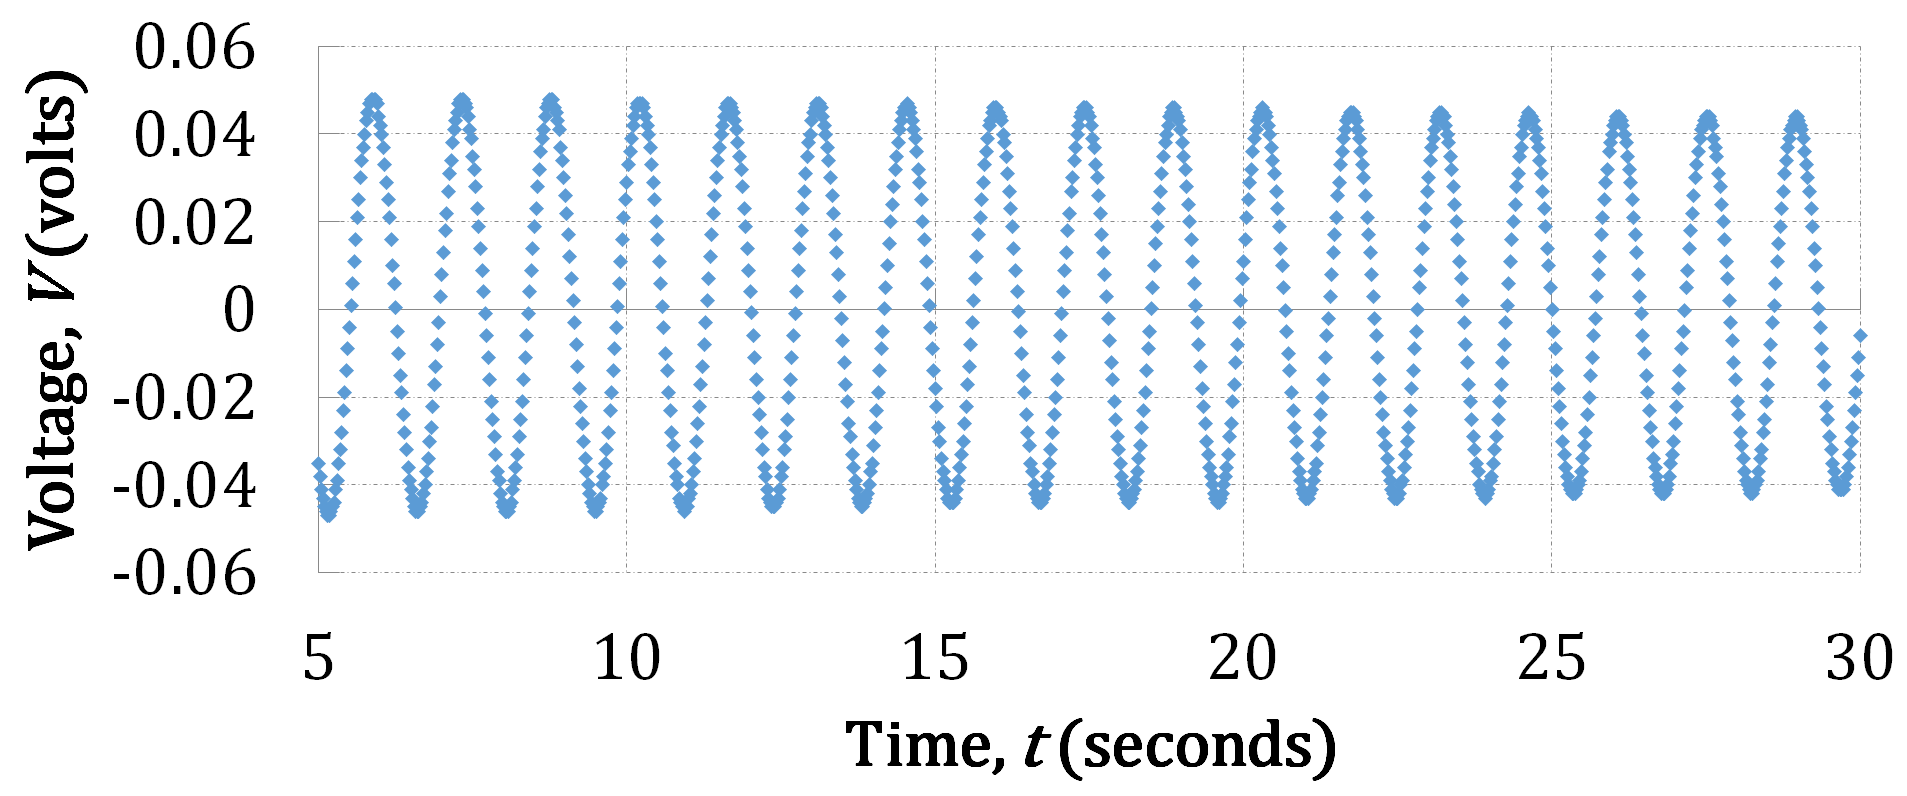
\includegraphics[width=2.9in]{UndampedOsc.png}
    \caption{\textit{Measuring Frequency of Undamped Oscillation.} Each blue diamond represents measured voltage displayed on force sensor at given time interval during oscillation.}
\end{figure}

\noindent Viewing the various maxima of the voltage output, we can then solve for the period of the oscillation by finding the elapsed time interval between each maxima and dividing that value by the number of elapsed maxima minus 1. We then take the inverse of the period to solve for frequency.

\footnotesize
\begin{equation}
f_0 = \bigg (\frac{\Delta t}{n-1} \bigg )\textsuperscript{-1}
\end{equation}
\normalsize

\noindent To normalize the data, we repeat this process for multiple ranges of extrema and solve for the uncertainty of our calculated frequency by using Equation ii.13 from the Lab Manual:

\footnotesize
\begin{equation}
\delta f = \frac{\sigma_f}{\sqrt{N}}
\end{equation}
\normalsize

\noindent Where $\sigma_f$ is the sample standard deviation and $N$ is the number of data points.$\textsuperscript{[1]}$ Using these equations, we estimate $f_0$ for the undamped oscillation to be (0.6936 $\pm$ 0.0002) Hz, which falls within the uncertainty range of our initial estimated $f_0$. We then repeat the process with the damped oscillation and solve for $f_0$ for the damped oscillation.

\begin{figure}[!htbp]
    \centering
    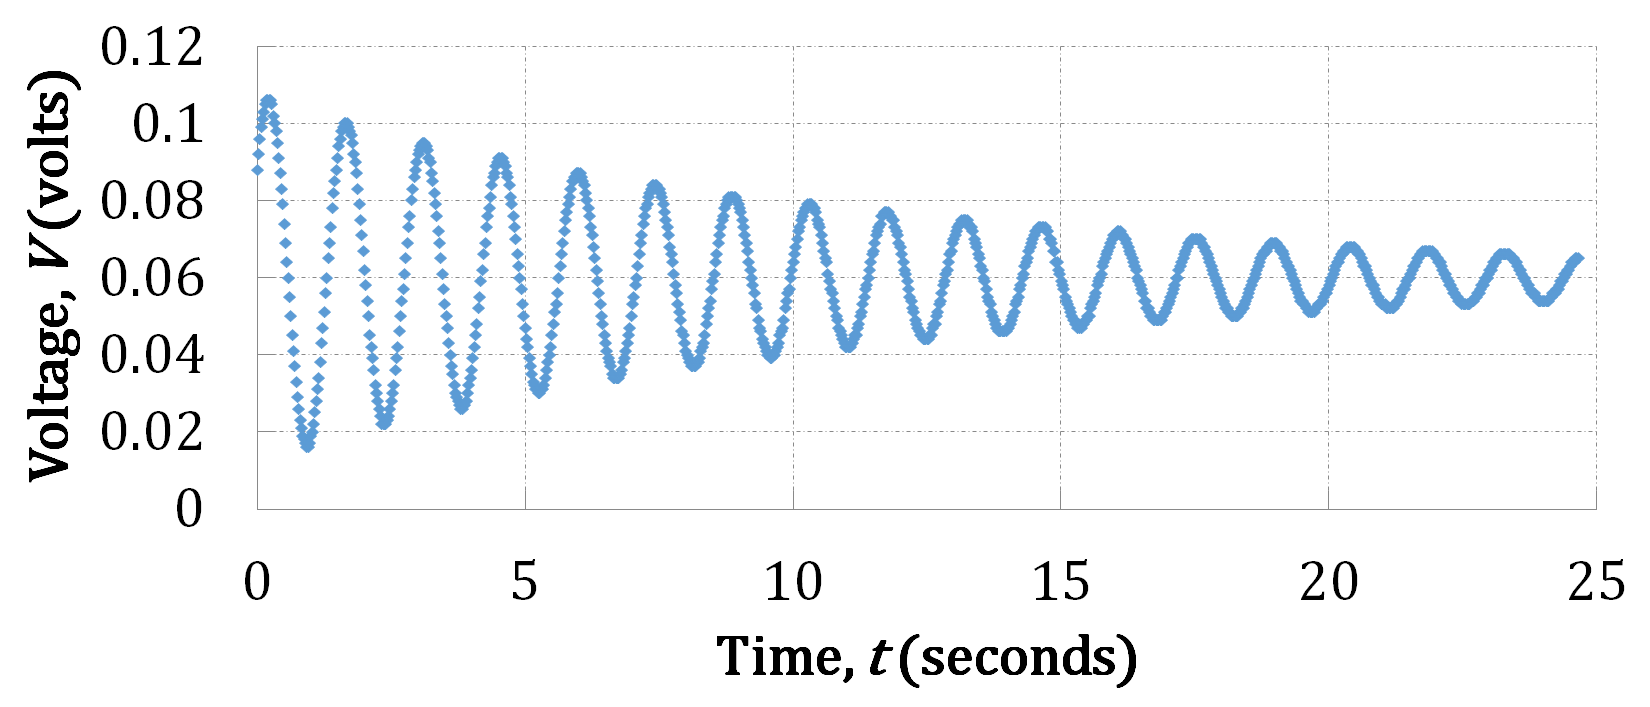
\includegraphics[width=2.9in]{DampedOsc.png}
    \caption{\textit{Measuring Frequency of Damped Oscillation.} Each blue diamond represents measured voltage displayed on force sensor at given time interval during oscillation.}
\end{figure}

\noindent Using Figure 3 above, we estimate $f_0$ of the damped oscillation to be (0.6926 $\pm$ 0.0018) Hz. As anticipated by the Lab Manual, the uncertainty of the damped oscillation is greater as the signal-to-noise ratio becomes worse as the amplitude decreases.$\textsuperscript{[1]}$ The frequency nonetheless still falls within the uncertainty of the initial estimated frequency of the system, given by Equation 3.

\hfill

\noindent We then test to see whether the damping can be described by a velocity-dependent damping force. To do so, we begin by removing the voltage offset from the damped oscillation data. We find the voltage offset to be approximately 0.0612 volts with a downard trend of 0.00009 volts per second. Using this information, we can describe the centered voltage as the following:

\footnotesize
\begin{equation}
V\textsubscript{centered} = V_0 - 0.0612 + 0.0001t
\end{equation}
\normalsize

\noindent With $t$ being the corresponding point in time at which the voltage was recorded. 

\noindent Using the centered data, we can then plot the ratios of successive maxima to test for whether damping is proportional to velocity.

\begin{figure}[!htbp]
    \centering
    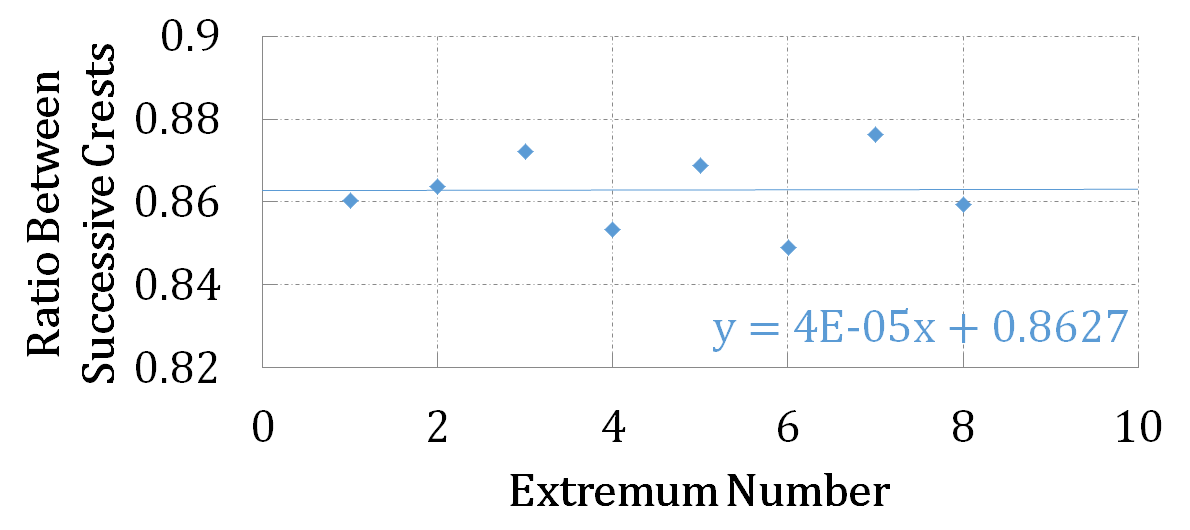
\includegraphics[width=2.9in]{Ratio.png}
    \caption{\textit{Confirmation of Velocity-Dependent Damping.} The blue line is a linear fit to the data, which in the event that the damping is velocity-dependent, should ideally have a slope of zero. It is given by the equation $y = 0.00004x + 8627$.}
\end{figure}

\noindent Averaging these values and finding their sample standard deviation per Equation ii.12 from the Lab Manual, we find that the ratio between amplitude of crests, $\frac{V(t+T)}{V(t)}$, is 0.863 $\pm$ 0.009.$\textsuperscript{[1]}$ We can then solve for the damping time, $\tau$, as defined in Equation 1, using the following:

\footnotesize
\begin{equation}
\tau = -\frac{T}{\text{ln}\Big [\frac{V(t+T)}{V(t)}\Big ]}
\end{equation}
\normalsize

\noindent We find $\tau = (4.72 \pm 0.35)$s via Equation 8 above and Equation ii.13 from the Lab Manual. Therefore using the following relationships and Equation ii.23 from the Lab Manual, we can solve for $Q$, the quality factor, of the resonance:$\textsuperscript{[1]}$

\footnotesize
\begin{align}
b &= \frac{2m}{\tau} \\
Q &= \frac{\sqrt{km}}{b} \\
\delta Q &= Q\sqrt{\bigg (\frac{\delta b}{b}\bigg )^2 + \bigg (\frac{\delta k}{2k}\bigg )^2 + \bigg (\frac{\delta m}{2m}\bigg )^2}
\end{align}
\normalsize

\noindent Plugging in the values for Equation 10 and 11, we find $Q$ = 10.28 $\pm$ 0.22. Using $Q$, we can now solve for $f\textsubscript{damped}$ using the following:

\footnotesize
\begin{align}
f\textsubscript{damped} &= f_0\sqrt{1-\frac{1}{4Q^2}} \\
\delta f\textsubscript{damped} &= f\textsubscript{damped}\sqrt{\bigg (\frac{\delta f_0}{f_0}\bigg )^2 + \bigg (\frac{\delta Q}{Q}\bigg )^2}
\end{align}
\normalsize

\noindent Therefore, $f\textsubscript{damped} = (0.6918 \pm 0.0149)$ Hz.

\hfill

\noindent A second method that can be used to obtain $Q$ is by taking the Fourier transform of the time-domain signal. Using the Capstone algorithm, we can then generate a plot of the frequency content in the time-domain signal.

\begin{figure}[!htbp]
    \centering
    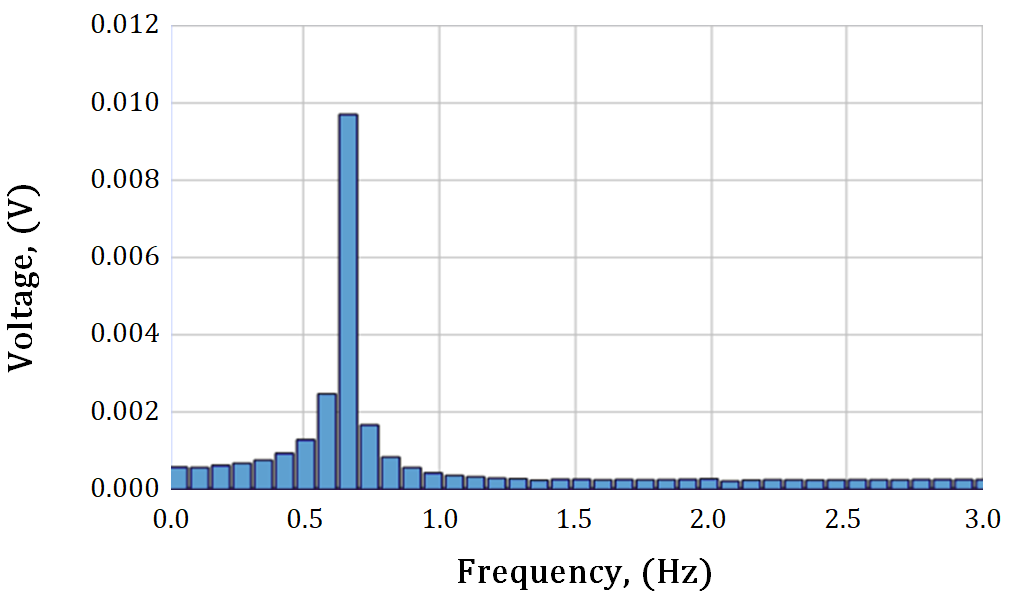
\includegraphics[width=2.9in]{FFT.png}
    \caption{\textit{FFT of Damped Oscillation.} The blue bars represent a frequency-domain representation of the data show in Figure 3.}
\end{figure}

\noindent Using the Figure 5 above, we can define the following equation:

\footnotesize
\begin{equation}
Q = \frac{f_0}{\Delta f}
\end{equation}
\normalsize

\noindent $\Delta f$ is defined as the width of the FFT curve when it is at a height of $\frac{1}{\sqrt{2}}$ of the maximum. Viewing the figure above, we define $\Delta f \approx 0.08$ Hz. Plugging in the $f_0$ and $\Delta f$ into Equation 14, we find $ Q= 8.6575$. While there is a significant difference in the value of the calculated $Q$, when we plug the FFT value of $Q$ back into Equation 12, we find the calculated frequency to be 0.6914 Hz. The small difference of the calculated $f\textsubscript{damped}$ implies a large $Q$ value is necessary to affect the frequency.

%------------------------------------------------

\section{Discussion}
\noindent From the experimental tests, we find that the predicted values for the frequencies of oscillation to be within the error values of the measured frequencies of oscillation from the experiment. 

\hfill

\noindent For the experimental value of the $f\textsubscript{damped}$, we find a small discrepancy in the value when compared with the predicted value of $f\textsubscript{damped}$: the two values being $(0.6918 \pm 0.0149)$ Hz and (0.6926 $\pm$ 0.0018) Hz, respectively.  The lower value of the experimental $f\textsubscript{damped}$ can be attributed to air resistance. Air resistance is a velocity dependent force; therefore, air resistance causes a higher value of $b$ which in turn causes a lower value of $Q$. Consequently, this then leads to a lower calculated experimental value of $f\textsubscript{damped}$.

\hfill

\noindent Air resistance, as discussed above, serves as a primary source of systematic uncertainty within this experiment. For both undamped and damped oscillations, the force of air resistance will decrease the amplitude of oscillation. This effect is visible in Figure 2, which should have no change in amplitude should the experiment have been performed under ideal conditions. However, a small change in amplitude can be observed. In the case of the damped oscillation, air resistance skews the calculated experimental values in the manner described above. This source of uncertainty can be eschewed by performing the experiment in an environment such as a vacuum.

\hfill

\noindent Another prominent source of systematic uncertainty for this experiment lies in the fact that the mass of the spring is not factored into our calculations. Since the spring mass is not taken into account for the calculation of the $Q$ value, the value that is calculated is skewed towards a lower value, which is then reflected in a lower value for predicted frequency. This source of error can be mitigated by using a weight that has significantly more mass than the spring.

\hfill

\noindent Interestingly enough, the thermal noise that served as the damping force in this experiment serves as a major obstacle in many fields by limiting the precision of measurement.$\textsuperscript{[3]}$  Application of the research spectrum of damped oscillations include the study of ultracold systems such as Bose-Einstein condensates and their accompanying phenomena.$\textsuperscript{[4]}$ In manufacturing, efficiency of the damping of harmonic oscillators in applications such as shock absorbers also remains a field of study and research.$\textsuperscript{[5]}$


%----------------------------------------------------------------------------------------
%	REFERENCE LIST
%----------------------------------------------------------------------------------------

\begin{thebibliography}{99} % Bibliography - this is intentionally simple in this template

\bibitem{1}
Campbell, W. C. \textit{et al}. Physics 4AL: Mechanics Lab Manual (ver. August 31, 2017).
(Univ. California Los Angeles, Los Angeles, California).

\bibitem{2}
Vitorino, M. \textit{et al}. Effect of sliding friction in harmonic oscillators. 
\textit{Sci. Rep.} \textbf{7}, 3726; doi:10.1038/s41598-017-03999-w (2017).


\bibitem{3}
Smith, N. D. A technique for continuous measurement of the quality factor of mechanical oscillators.
\textit{Review of Scientific Instruments} \textbf{86}, 053907; doi:10.1063/1.4920922 (2015).

\bibitem{4}
Wang, Y. \textit{et al}. Sonic horizon formation for oscillating Bose-Einstein condensates in isotropic harmonic potential. 
\textit{Sci. Rep.} \textbf{6}, 38512; doi: 10.1038/srep38512 (2016).

\bibitem{5}
Ryabov, I.V. \textit{et al}. Efficiency of Shock Absorber in Vehicle Suspension.
\textit{International Conference on Industrial Engineering, ICIE 2016}. Procedia Engineering 150, 354 - 362 
(Volgograd State Technical University, Lenin Avenue, 28, Volgograd, 400005, Russia, 2016).
\end{thebibliography}

%----------------------------------------------------------------------------------------

\end{document}
